%!TEX program = xelatex
% 完整编译: xelatex -> biber/bibtex -> xelatex -> xelatex
\documentclass[lang=cn,a4paper,citestyle=gb7714-2015, bibstyle=gb7714-2015]{elegantpaper}

\title{NSGA-II算法}

\author{姜孟冯\textsuperscript{1,2}}
\institute{(1.中国矿业大学,徐州;\ 2.应急管理部信息研究院,北京)}
\date{\zhtoday}

%%%%%%%%%%%%%%%%%%%%%%%%%%%%%%%%%%%%%%%%%%%%%%%%%%%%%%%%%%%%%%%%%%%%%
% PACKAGES                                                          %
%%%%%%%%%%%%%%%%%%%%%%%%%%%%%%%%%%%%%%%%%%%%%%%%%%%%%%%%%%%%%%%%%%%%%
\usepackage{amssymb}
\usepackage{optidef}
%\usepackage{tabularray}
\usepackage{biblatex}
\addbibresource[location=local]{reference.bib} % 参考文献
\usepackage{graphicx}
%\usepackage{wrapfig}
\usepackage{subcaption}
%%%%%%%%%%%%%%%%%%%%%%%%%%%%%%%%%%%%%%%%%%%%%%%%%%%%%%%%%%%%%%%%%%%%%%
% STYLE ENVIRONMENT                                                  %
%%%%%%%%%%%%%%%%%%%%%%%%%%%%%%%%%%%%%%%%%%%%%%%%%%%%%%%%%%%%%%%%%%%%%%

%%%%%%%%%%%%%%%%%%%%%%%%%%%%%%%%%%%%%%%%%%%%%%%%%%%%%%%%%%%%%%%%%%%%%%
% MY COMMANDS                                                        %
%%%%%%%%%%%%%%%%%%%%%%%%%%%%%%%%%%%%%%%%%%%%%%%%%%%%%%%%%%%%%%%%%%%%%%
\newcommand{\R}{\mathbf{R}}
\newcommand{\C}{\mathbf{C}}
\newcommand{\F}{\mathbf{F}}
\newcommand{\U}{\mathit{U}}
\newcommand{\V}{\mathit{V}}
\newcommand{\W}{\mathit{W}}
\newcommand{\poly}{\mathcal{P}}
\newcommand{\espace}{\mathcal{L}}
\newcommand{\expect}{\mathcal{E}}
\newcommand{\mat}{\mathcal{M}}
\newcommand{\mtxA}{\mathcal{A}}
\DeclareMathOperator{\Span}{span}
\DeclareMathOperator{\Real}{Re}
\DeclareMathOperator{\Imag}{Im}
\DeclareMathOperator{\Null}{null}
\DeclareMathOperator{\Range}{range}
\newcommand{\ph}{\phantom{+x_0}}
\newcommand{\mycite}[1]{\textsuperscript{\parencite{#1}}}
\newcommand{\link}[1]{\href{#1}{#1}}

%\newcommand{\bigO}{\mathcal{O}}
%\newcommand{\mat}{\mathcal{M}}
%\newcommand{\defeq}{\vcentcolon=}
%\newcommand{\restr}[1]{|_{#1}}

%%%%%%%%%%%%%%%%%%%%%%%%%%%%%%%%%%%%%%%%%%%%%%%%%%%%%%%%%%%%%%%%%%%%%%
% SECTION SETTINGS                                               %
%%%%%%%%%%%%%%%%%%%%%%%%%%%%%%%%%%%%%%%%%%%%%%%%%%%%%%%%%%%%%%%%%%%%%%
%\renewcommand{\thesubsection}{\thesection\Alph{subsection}}
%\renewcommand{\thesubsubsection}{\arabic{subsubsection}}

%%%%%%%%%%%%%%%%%%%%%%%%%%%%%%%%%%%%%%%%%%%%%%%%%%%%%%%%%%%%%%%%%%%%%%
% DOCUMENT                                                           %
%%%%%%%%%%%%%%%%%%%%%%%%%%%%%%%%%%%%%%%%%%%%%%%%%%%%%%%%%%%%%%%%%%%%%%
\begin{document}

    \maketitle

    \section{算法背景}
    \subsection{多目标优化问题}
    \textbf{多目标优化问题(MOP)}是涉及多个目标函数同时优化的数学问题。
    需要在两个或多个相互冲突的目标之间进行权衡的情况下作出最优决策。

    \begin{definition}
        多目标优化问题(multi-objective optimization problem,简称MOP)
        \begin{mini*}|s|
            {}
            {y = (f_1(x),f_2(x), \dots , f_r(x))}
            {}
            {}
            \addConstraint{g_i(x)}{\geq 0,i=1,2,\dots,k}
            \addConstraint{h_i(x)}{= 0,i=1,2,\dots,l}
        \end{mini*}
        这里$x=(x_1,x_2,\dots,x_n)$是一个n维决策向量,向量空间$X\subseteq\R^n$,y是一个r维目标向量$y\in \R^r$,f为目标函数,g和h分别为不等式约束与等式约束条件,记问题的可行解集为$\Omega$。
    \end{definition}

    \begin{definition}
        Pareto支配(Pareto Dominance)\\
        设$a,b\in \Omega$,a支配b,记为 $a \prec b$ ,当且仅当以下条件同时成立
        $$\forall{i}\in\{1,2,\dots,r\}, f_i(a) \leq f_i(b)\ \ \text{且}\ \ \exists {j} \in \{1,2,...,r\}, f_j(a)<f_j(b)$$
    \end{definition}


    \begin{definition}
        Pareto最优解集(Pareto Optimal Set)\\
        如果一个可行解$x^*\in \Omega$被称之为Pareto optimal solution, 当且仅当 $x^∗$ 不被其他的解支配。易见$x^*$往往不是一个,用$PS^*=\{x^*\}$表示最优解集
        $$PS^*=\{x^*\}=\{x\in\Omega|\neg\exists X'\in\Omega,f_j(x')\leq f_j(x) (j=1,2,\dots,r)\} $$
    \end{definition}

    \begin{definition}
        Pareto边界(Pareto Optimal Front,简称PF)\\
        Pareto Optimal Set 中每个解对应的目标值向量组成的集合称之为Pareto Front(如\figref{fig:pf}所示)。
        $$PF^*=\{f(x) = (f_1(x),f_2(x), \dots, f_r(x))|x\in PS^*\}$$
    \end{definition}
    \begin{figure}[!h]
        \centering
        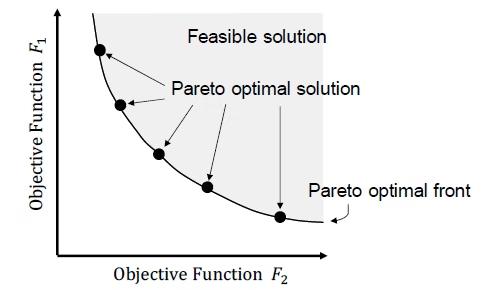
\includegraphics[width=0.4\textwidth]{ParetoFront}
        \caption{Pareto边界示意图}
        \label{fig:pf}
    \end{figure}


    \subsection{多目标进化算法与分类}
    \textbf{多目标进化算法(Multi-objective Evolutionary Algorithm,简称MOEA)}是一种非常有效的解决多目标优化问题(MOP)的方法。1989年,David Goldberg在其著作《Genetic Algorithm in Search, Optimization and Machine Learning\mycite{goldberg1989genetic}》中,提出了用进化算法实现多目标的优化技术,对多目标进化算法的研究具有重要的方向性指导意义。根据不同的进化机制,MOEA可以分为三类\mycite{郑金华2017多目标进化优化}:
    \begin{enumerate}
        \item 基于分解的MOEA:权重聚合函数、切比雪夫聚合、基于惩罚的边界交叉、MOEA/D
        \item 基于支配关系的MOEA:NSGA-II、NPGA、SPEA2、PESA、PAES、MOMGA、mBOA、MMOGA
        \item 基于指标的MOEA:SMS-EMOA、IBEA、HypE
    \end{enumerate}

    \subsection{NSGA-II算法}
    1994年,Srinivas和Deb提出了NSGA(nondominated sorting genetic algorithm)\mycite{NSGA},可以有效求解MOP问题,但仍存在一些不足之处:(1)缺少最优个体保留机制(2)共享参数大小不易确定(3)构造非支配集的时间复杂度高$(O(rN^3))$。2000年,Deb等对算法进行优化,提出了NSGA-II\mycite{NSGA2prototype},2002年又对其中的非支配集排序方法进行了改进\mycite{NSGA2},把时间复杂度提高到$(O(rN^2))$,但只适用于处理低维优化问题(维数小于等于3)。2013年,Deb等又提出了NSGA-III\mycite{NSGA3},用以解决高维数问题。

    本文主要集中讨论NSGA-II算法。

    \section{NSGA-II算法原理及框架}
    \subsection{算法框架}
    NSGA-II算法是一种多目标进化算法,全称是Elitist Non-dominated Sorting Genetic Algorithm(精英非支配排序遗传算法),NSGA-II的主要特征有三点:
    \begin{itemize}
        \item 基于快速非支配排序的等级(rank)划分方法
        \item 计算拥挤度(crowding-distance)的方法
        \item 用以上二者构建的偏序比较算子代替共享参数(sharing fuction)
    \end{itemize}

    NSGA-II算法基于遗传算法的逐代进化思想,开始时随机产生一个父代种群$P_t$,然后利用选择、交叉、变异的方式生成临时子代$Q_t$,利用“非支配排序”与“拥挤度计算”来对父子种群中的每个个体进行适应度评估,选出新一代精英个体作为新的父代$P_{t+1}$,如此不断循环进化,直到满足结束条件。

    NSGA-II基本流程框架如\figref{fig:nsga-ii-structure}所示:
    \begin{figure}[!h]
        \centering
        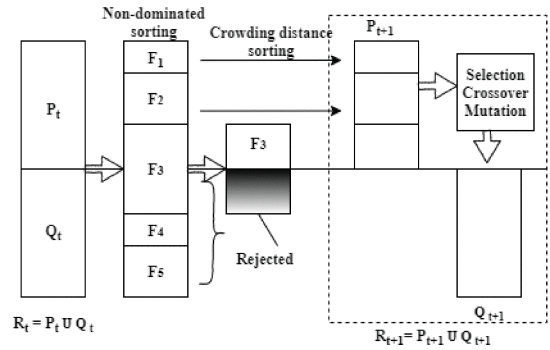
\includegraphics[width=0.5\textwidth]{nsga-ii-structure}
        \caption{NSGA-II流程示意图}
        \label{fig:nsga-ii-structure}
    \end{figure}

    \subsection{快速非支配集排序方法}
    在NSGA中,非支配集排序方法的时间复杂度是$(O(rN^3))$,NSGA-II改进了非支配集的构造方式。设向量$S_p$表示个体p所支配的个体集合,标量$n_p$表示能够支配当前个体p的个数,即有
    $$S_p=\{q|p\prec q,p,q\in \text{种群}P\},\quad n_p=|\{q|q\prec p,p,q\in \text{种群}P\}|$$

    可利用上述变量及个体间的支配关系对种群P进行划分,输出$F_i(i=1,2,...,m)$.
    $$F_i=\{q|n_q-i+1=0,q \in P\}$$

    \begin{figure}[!h]
        \centering
        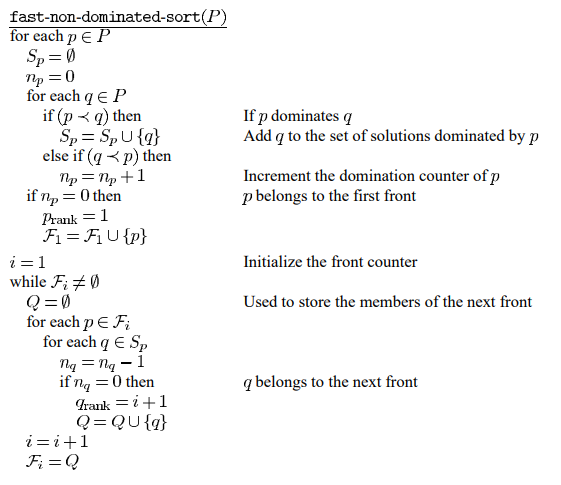
\includegraphics[width=0.7\textwidth]{fast-non-dominated-sort}
    \end{figure}

    算法fast-non-dominated-sort由两部分组成,第一部分用于计算$S_p$与$n_p$并构造$F_1$,种群规模为N,目标数为r时,时间复杂度为$O(rN^2)$。第二部分用于求解$F_i$,最坏情况下存在N层边界,即m=N,时间复杂度为$O(N^2)$。由此可知,算法的时间复杂度为$O(rN^2)+O(N^2)=O(rN^2)$。

    \subsection{拥挤度计算方法}
    设下标为i的个体的拥挤度记为$i_{distance}$,目标函数值记为$f_j(x_i)$,用$f_j^{max}$与$f_j^{min}$分别表示目标函数的最大最小值,则拥挤度计算可使用以下公式:

    边界上的点:$i_{distance}=\infty$

    边界以外的点:$i_{distance}= \sum\limits_{j=1}^r(\dfrac{f_j(x_{i+1}) - f_j(x_{i-1})}{f_j^{max} - f_j^{min}})$

    \begin{figure}[!h]
        \centering
        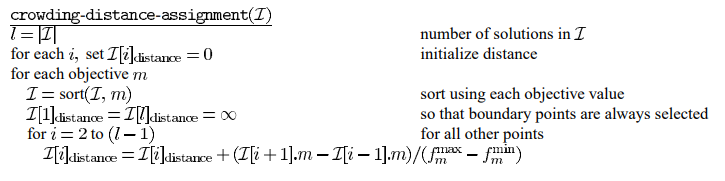
\includegraphics[width=0.9\textwidth]{crowding-distance}
    \end{figure}

    算法crowding-distance-assignment描述了计算个体拥挤度的过程,此过程需要按每个子目标函数值进行排序,最坏情况下对r个子目标进行排序,时间复杂度为$O(rN\log N)$,而计算拥挤度本身的时间为$O(rN)$,由此可知算法的时间复杂度为$O(rN\log N)$。

    \subsection{精英保留策略}
    NSGA-II的适应度评估过程中,考虑了个体i的两个属性,非支配排序等级与拥挤度,记作$i_{rank}$与$i_{distance}$,二者可以构成一个偏序关系$\prec_n$。

    \begin{definition}
        个体之间的偏序关系$\prec_n$
        $$i\prec_nj\quad if(i_{rank}<j_{rank})\quad or\quad ((i_{rank}=j_{rank})\quad and\quad  (i_{distance} > j_{distance}))$$
    \end{definition}
    利用该偏序关系,可以构建偏序比较算子,该算子避免了任何用户定义的参数,同时改善了计算复杂度。
    如此可定义精英保留策略如下:
    \begin{enumerate}
        \item 将父代种群$P_t$通过选择、交叉、变异策略生成子代种群$Q_t$
        \item 把$P_t$和$Q_t$合成种群$R_t$
        \item 根据偏序关系$\prec_n$将种群$R_t$中的个体逐个放入新的父代种群$P_{t+1}$,直到填满。
    \end{enumerate}

    \section{算法步骤及实现}

    \subsection{基本步骤}
    NSGA-II主循环算法可用伪代码描述如下:

    \begin{figure}[!h]
        \centering
        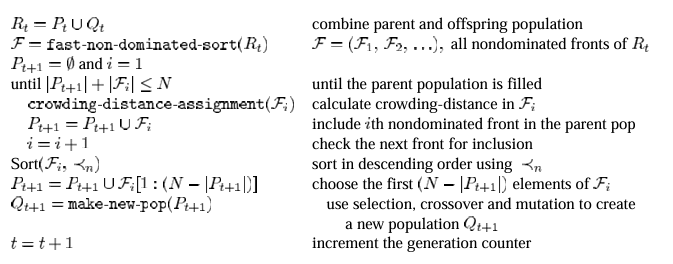
\includegraphics[width=0.8\textwidth]{nsga-ii-algorithm}
    \end{figure}

    具体来说,NSGA-II使用快速非支配排序来保证收敛性,并且利用拥挤距离来保证分布性。其主要时间开销由三部分组成:
    \begin{enumerate}
        \item 构造非支配集划分(fast-non-dominated-sort):$O(r(2N)^2)$
        \item 拥挤度计算(crowding-distance-assignment):$O(r(2N)\log (2N))$
        \item 构造偏序集(sort on $\prec_n$):$O(2N\log2N)$
    \end{enumerate}

    综合考虑,算法的时间复杂度为:$O(rN^2)$。

    \subsection{参数设置}
    NSGA-II算法的参数设置对算法的性能有重要影响。主要参数包括:
    \begin{itemize}
        \item 种群规模(N):控制种群中个体的数量。较大的种群规模可以提供更广泛的搜索空间,但计算成本更高。
        \item 最大进化代数(MaxGen):控制算法运行的代数。较大的最大进化代数可以提高算法的收敛性,但计算成本也更高。
        \item 交叉概率(Pc):控制交叉算子应用的概率。较高的交叉概率可以促进种群多样性,但可能导致过早收敛。
        \item 变异概率(Pm):控制变异算子应用的概率。较高的变异概率可以引入新的个体,但可能破坏种群的收敛性。
    \end{itemize}
    %
    \subsection{开源实现}

    \begin{enumerate}
        \item[C]nsga2: \link{https://www.iitk.ac.in/kangal/codes.shtml}
        \item[Java]MOEA Framework:\link{https://github.com/MOEAFramework/MOEAFramework}
        \item[Python]pymooo: \link{https://github.com/anyoptimization/pymoo}
        \item[Julia]Metaheuristics: \link{https://github.com/jmejia8/Metaheuristics.jl}
        \item[R]rmoo: \link{https://github.com/Evolutionary-Optimization-Laboratory/rmoo}
        \item[Rust]Optirustic: \link{https://github.com/s-simoncelli/optirustic}
        \item[C\#]MOEAs: \link{https://github.com/qshzhang/MOEAs}
    \end{enumerate}

    可见,NSGA-II算法作为多目标优化(MOO)领域的经典算法,被众多编程语言予以实现,方便后人研究与改进。
    \section{算法应用}
    NSGA-II算法应用非常广泛,

    \subsection{科学问题研究}

    Shanu Verma等在2021年对NSGA-II相关的论文发表情况进行了分析\mycite{Verma2021},从Science Direct、Taylor \& Francis Online、Wiley Online Library、Springer与IEEE Xplore等在线数据库上选出了169篇NSGA-II论文。按照多目标组合优化问题的各类子问题进行统计,得出结果如\figref{fig:nsga-ii-paper}所示。调度问题(占比42\%)是最适用NSGA-II算法最解决的多目标优化问题(MOCOP)中最为常见的,紧随其后的是分配问题(占比17\%)、其他问题(占比11\%)、指派问题(占比11\%)、车辆路径问题(VRP)(占比8\%)、背包问题(占比7\%)以及旅行商问题(TSP)(占比4\%)。在应用算法方面,改进后的NSGA-II算法(占比58\%)被最广泛地使用,其次是混合NSGA-II算法(占比34\%),而传统的NSGA-II算法使用较少,仅占8\%。
    \begin{figure}[!h]
        \centering
        \begin{subfigure}[h]{0.4\textwidth}
            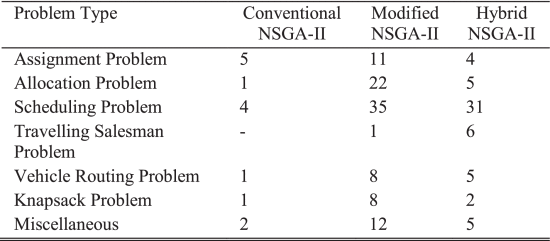
\includegraphics[width=\textwidth]{nsga-ii-paper-1}
        \end{subfigure}
        \begin{subfigure}[h]{0.4\textwidth}
            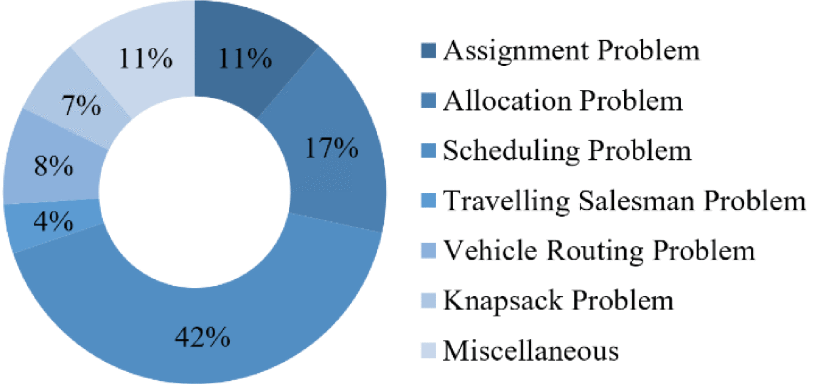
\includegraphics[width=\textwidth]{nsga-ii-paper-2}
        \end{subfigure}
        \caption{NSGA-II研究论文按问题分类}
        \label{fig:nsga-ii-paper}
    \end{figure}

    若以年为维度,如\figref{fig:nsga-ii-years}所示,可见一直至2020年,NSGA-II的研究热度持续上涨。

    \begin{figure}[!h]
        \centering
            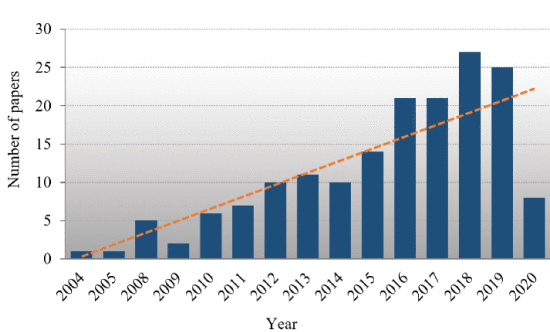
\includegraphics[width=0.6\textwidth]{nsga-ii-years}
        \caption{NSGA-II研究论文按年的研究热度}
        \label{fig:nsga-ii-years}
    \end{figure}

    \subsection{机械设计与制造}

    机械设计与制造是NSGA-II算法最常见的应用领域之一。在机械设计中,往往需要同时考虑多个目标,如成本、性能、可靠性等。NSGA-II算法可以有效地处理多目标优化问题,找到满足所有目标约束的最佳解决方案。使用NSGA-II算法的案例非常之多,比如:车用行星齿轮成形工艺\mycite{DYJE202410008}、缠绕过程多目标工艺\mycite{FUHE202410040}、杯状纵磁触头结构\mycite{DGJS202223015}等等。

    \subsection{环境与资源分配}

    环境与资源分配优化是NSGA-II算法的另一个重要应用领域。在资源分配问题中,需要在有限的资源约束下,将资源分配给多个目标,这正是经典的MOP问题,比如供水系统规划\mycite{SDNY202307032}\mycite{SDNY202212043}、供电系统规划\mycite{KXJS202214018}\mycite{JZDF202301007}、土地资源利用规划\mycite{STBC202402007}\mycite{CHKD202208018}、充电站选址\mycite{ZZDZ20241024001}等,都可以用NSGA-II算法有效地解决。


    \subsection{电子与电气工程}
    在电子与电气工程方面,NSGA-II的应用也比较广泛。随着硅片上集成的晶体管数量迅猛增加,基于IP核的片上系统(systemonachip,SOC)已成为VLSI实现技术发展的趋势。目前SOC的系统设计主要采用基于可编程IP核的配置、仿真与封测,所有功能验证完毕后才产生物理芯片。由于IP核的多样性及其可优化参数的矛盾性,使得SOC的设计空间极其复杂。SOC系统的主要任务之一就是针对具体的应用在可能的设计空间中找到一组满足设计约束的IP可行配置集,或者是找到功率/性能平衡面,把功耗和执行时间的最小化作为优化目标。案例如:监测天线部署优化\mycite{XDKD202105027}、阵列芯片的微通道结构参数优化\mycite{HXDY202404012}、三模冗余软错误防护技术\mycite{DZYX202405006}等。


    \nocite{*}
    \printbibliography[heading=bibintoc, title=\ebibname]
\end{document}
